\documentclass[10pt]{standalone}
\usepackage{amsmath}
\usepackage{pgf,tikz}
\usetikzlibrary{calc}
\usepackage{mathrsfs}
\usetikzlibrary{arrows}
\pagestyle{empty}
\begin{document}
	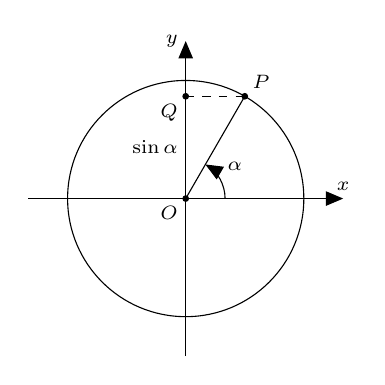
\begin{tikzpicture}[>=triangle  45]
	\tikzset{samples=600}
	\pgfmathsetmacro{\raggio}{1.5};
	\pgfmathsetmacro{\angolo}{60};
	\pgfmathsetmacro{\y}{3};
	\pgfmathsetmacro{\XM}{\raggio};
	\pgfmathsetmacro{\sraggio}{1.0*\raggio};
	
\begin{scriptsize}
	\coordinate [label=below left:$O$] (oo)  at (0,0);
	\draw[->] (-\raggio-0.5,0) -- (\raggio+0.5,0) node[above] {$x$} ;
	\draw[->] (0,-\raggio-0.5) -- (0,\raggio+0.5) node[left] {$y$} ;
	\draw (oo) circle (\raggio) ;
	\filldraw[black] (oo) circle(1pt);
	\coordinate [label=above right:$P$] (P) at  ({\raggio*cos(\angolo)},{\raggio*sin(\angolo )});
	\coordinate[label=below left:$Q$] (Q) at (0,{\raggio*sin(\angolo)});
	\draw (oo)  -- (Q) node[midway,left]{$\sin\alpha$} ;
	\draw[->] (\sraggio/\y,0 ) arc (0:\angolo:\sraggio/\y);
	\draw (\angolo/2:\sraggio/\y) node[ above right]  {$\alpha$};
	\filldraw[black] (Q) circle(1pt);
	\filldraw[black] (P) circle(1pt);
	\draw (oo)-- (P) ;
	\draw[dashed](Q)-- (P) ;
\end{scriptsize}		
	\end{tikzpicture}
\end{document}